\section{Arnoldi正交化}
\label{sec:ls-arnoldi}

第~\ref{sec:ls-krylov-subspaces}节的选解准则都要在$\mathcal K_k(\bm A,\bm r_0)$中计算，而幂向量$\bm r_0,\bm A\bm r_0,\ldots$随次数增加趋于同一方向，不宜直接作基。对一般方阵，\term{Arnoldi正交化}（Arnoldi process）逐个生成这个子空间的一组标准正交基，并把$\bm A$在子空间上的作用记录为一个上Hessenberg小矩阵。

下面先说明它的任务与正交化方法，再写出计算过程，然后分析所得结果的含义，最后说明它怎样用于求解方程。后两节的Lanczos过程与Golub--Kahan双对角化分别是它在对称矩阵与长方矩阵上的变形。

\subsection{主要思想}

给定方阵$\bm A\in\mathbb R^{d\times d}$，不要求对称，只假定$\bm A$乘向量容易计算；再给定初始残差$\bm r_0\ne\bm 0$与迭代步数$k$。Arnoldi正交化要生成一组标准正交向量$\bm v_1,\ldots,\bm v_k$，使对每个$j\le k$，前$j$个向量张成$\mathcal K_j(\bm A,\bm r_0)$。

\paragraph{修正Gram--Schmidt正交化}

第一个向量取初始残差的方向，
\begin{equation}
 \bm v_1=\frac{\bm r_0}{\lVert\bm r_0\rVert_2},
 \label{eq:ls-arnoldi-start}
\end{equation}

设已有标准正交的$\bm v_1,\ldots,\bm v_j$，它们张成$\mathcal K_j$。$\bm v_j$在$\bm A^{j-1}\bm r_0$上的系数非零，所以
\[
  \mathcal K_{j+1}=\mathcal K_j+\operatorname{span}\{\bm A\bm v_j\} ,
\]
$\mathcal K_{j+1}$比$\mathcal K_j$多出的方向来自$\bm A\bm v_j$。

于是先作$\bm w=\bm A\bm v_j$，再用第~\ref{sec:ls-qr-method}节的修正Gram--Schmidt把它在已有基向量上的分量逐个扣除，对$i=1,\ldots,j$依次计算
\begin{equation}
 h_{i,j}=\bm v_i^\top\bm w,\qquad \bm w\leftarrow\bm w-h_{i,j}\bm v_i .
 \label{eq:ls-arnoldi-coefficients}
\end{equation}
每个$h_{i,j}$都用已经扣除前面分量的当前$\bm w$求内积。

此前扣除的$\bm v_1,\ldots,\bm v_{i-1}$与$\bm v_i$正交，所以精确算术下这与$h_{i,j}=\bm v_i^\top\bm A\bm v_j$相同，有限精度下逐个扣除保持正交性更好。

扣除完毕后，余项$\bm w$与$\bm v_1,\ldots,\bm v_j$都正交，再把它归一化，
\begin{equation}
 h_{j+1,j}=\lVert\bm w\rVert_2,\qquad \bm v_{j+1}=\frac{\bm w}{h_{j+1,j}}\quad(h_{j+1,j}\ne0),
 \label{eq:ls-arnoldi-normalize}
\end{equation}
就得到下一个基向量。

把扣除的分量加回去，每个$\bm A\bm v_j$都是前$j+1$个基向量的组合：
\begin{equation}
 \bm A\bm v_j=\sum_{i=1}^{j+1}h_{i,j}\bm v_i .
 \label{eq:ls-arnoldi-column}
\end{equation}

\paragraph{与全部旧基向量耦合}
一般方阵的系数$h_{i,j}=\bm v_i^\top\bm A\bm v_j$（$i\le j$）通常都不为零，新向量与此前的全部基向量耦合：第$j$轮要与$\bm v_1,\ldots,\bm v_j$逐个求内积并扣除，整组基都须保存。第~\ref{sec:ls-lanczos}节将说明，$\bm A$对称时其中只有最近的两项非零，扣除可以缩短为三项递推。

\subsection{计算过程}

按上一小节的推导，Arnoldi正交化每轮作一次矩阵乘向量，把结果对已有基向量逐个扣除，再把余项归一化。下面写出计算中用到的变量、它们怎样初始化、每轮怎样更新。下面用例~\ref{ex:ls-stationary-running-example}的以下数据逐步演示：
\[
 \bm A=\begin{bmatrix}4&1\\1&3\end{bmatrix},\qquad \bm b=\begin{bmatrix}1\\2\end{bmatrix}.
\]
取$\bm x_0=\bm 0$，于是$\bm r_0=\bm b$，步数取$k=2$。

\paragraph{变量}
\begin{itemize}
 \item $\bm v_1,\ldots,\bm v_j\in\mathbb R^d$：已生成的标准正交基向量，全部保存。
 \item $\bm w\in\mathbb R^d$：工作向量，先存$\bm A\bm v_j$，再在原处逐个扣除已有分量，成为余项。
 \item $h_{1,j},\ldots,h_{j+1,j}$：第$j$轮的系数，即上Hessenberg矩阵$\overline{\bm H}_k$的第$j$列。
 \item $j$：轮次。
\end{itemize}

\paragraph{初始化}
把第一个基向量初始化为初始残差的方向，轮次初始化为$1$：
\[
 \bm v_1=\frac{\bm r_0}{\lVert\bm r_0\rVert_2},\qquad j=1 .
\]
例中$\lVert\bm r_0\rVert_2=\sqrt5$，
\[
 \bm v_1=\frac1{\sqrt5}\begin{bmatrix}1\\2\end{bmatrix}.
\]

\paragraph{每轮更新}
在第$j$轮：
\begin{enumerate}
 \item \textbf{乘矩阵。}计算
 \[
  \bm w=\bm A\bm v_j .
 \]
 例中第一轮
 \[
  \bm w=\bm A\bm v_1=(6,7)^\top/\sqrt5 .
 \]

 \item \textbf{逐个扣除已有分量。}按式~\eqref{eq:ls-arnoldi-coefficients}，对$i=1,\ldots,j$依次计算
 \[
  h_{i,j}=\bm v_i^\top\bm w,\qquad \bm w\leftarrow\bm w-h_{i,j}\bm v_i ,
 \]
 每个内积都用已扣除前面分量的当前$\bm w$。例中第一轮只有$i=1$：
 \[
  h_{1,1}=\frac{1\cdot6+2\cdot7}{5}=4,\qquad
  \bm w=\frac1{\sqrt5}\Bigl(\begin{bmatrix}6\\7\end{bmatrix}-4\begin{bmatrix}1\\2\end{bmatrix}\Bigr)=\frac1{\sqrt5}\begin{bmatrix}2\\-1\end{bmatrix}.
 \]

 \item \textbf{归一化。}按式~\eqref{eq:ls-arnoldi-normalize}计算
 \[
  h_{j+1,j}=\lVert\bm w\rVert_2,\qquad \bm v_{j+1}=\frac{\bm w}{h_{j+1,j}} .
 \]
 例中第一轮
 \[
  h_{2,1}=1,\qquad \bm v_2=\frac1{\sqrt5}\begin{bmatrix}2\\-1\end{bmatrix}.
 \]
 然后令$j\leftarrow j+1$，进入下一轮。
 
 例中第二轮先乘矩阵，得
 \[
  \bm w=\bm A\bm v_2=(7,-1)^\top/\sqrt5 ,
 \]
 再依次扣除两个方向：
 \[
  \begin{aligned}
  h_{1,2}&=\frac{7-2}{5}=1,&\qquad \bm w&=\frac1{\sqrt5}\begin{bmatrix}6\\-3\end{bmatrix};\\
  h_{2,2}&=\frac{12+3}{5}=3,&\qquad \bm w&=\bm 0 ,
  \end{aligned}
 \]
 于是$h_{3,2}=0$。

 \item \textbf{停止。}当$h_{j+1,j}=0$（实际中低于按输入尺度取定的阈值）时，$\bm A\bm v_j$已落在现有空间中，Krylov子空间不再扩张，不作归一化，退出迭代；否则做满$k$轮后退出。例中第二轮$h_{3,2}=0$，二维空间已经用尽，退出迭代。
\end{enumerate}
若扣除后的$\lVert\bm w\rVert_2$远小于扣除前的$\lVert\bm A\bm v_j\rVert_2$，说明发生了大量相消，余项可能已带有旧方向的成分。这时在归一化之前对已有基再投影一遍，得修正量$\delta_i=\bm v_i^\top\bm w$，令$\bm w\leftarrow\bm w-\delta_i\bm v_i$，并把它加回$h_{i,j}\leftarrow h_{i,j}+\delta_i$。

例中第一轮扣除前长度为$\sqrt{17}\approx4.12$，扣除后为$1$，相消不严重，不需再正交化。

最终得到标准正交基$\bm v_1,\bm v_2$与各轮系数组成的小矩阵。例中
\[
 \bm V_2=\frac1{\sqrt5}\begin{bmatrix}1&2\\2&-1\end{bmatrix},\qquad
 \bm H_2=\begin{bmatrix}h_{1,1}&h_{1,2}\\h_{2,1}&h_{2,2}\end{bmatrix}=\begin{bmatrix}4&1\\1&3\end{bmatrix},
\]
它们满足
\[
 \bm A\bm V_2=\bm V_2\bm H_2 .
\]

\subsection{算法分析}

\paragraph{基矩阵与投影矩阵}
把各步得到的标准正交基并排，记
\begin{equation}
 \bm V_k=[\bm v_1,\ldots,\bm v_k]\in\mathbb R^{d\times k}.
 \label{eq:ls-arnoldi-basis-matrix}
\end{equation}
它的行数是原矩阵的维数$d$，列数是迭代步数$k$。通常$k\ll d$，$\bm V_k$是一个瘦长矩阵：它的列张成$\mathcal K_k$，把$d$维空间中的这个$k$维子空间用$k$个坐标表示出来。

把$j=1,\ldots,k$的列关系~\eqref{eq:ls-arnoldi-column}按列并排写出，得到矩阵形式
\begin{equation}
 \bm A\bm V_k=\bm V_{k+1}\overline{\bm H}_k=\bm V_k\bm H_k+h_{k+1,k}\bm v_{k+1}\bm e_k^\top ,
 \label{eq:ls-arnoldi-relation}
\end{equation}
其中$\overline{\bm H}_k\in\mathbb R^{(k+1)\times k}$在$i\le j+1$处的元素为$h_{i,j}$、其余为零，$\bm H_k$是它去掉末行所得的$k$阶方阵。以$k=3$为例，
\[
 \bm A\begin{bmatrix}\bm v_1&\bm v_2&\bm v_3\end{bmatrix}
 =\begin{bmatrix}\bm v_1&\bm v_2&\bm v_3&\bm v_4\end{bmatrix}
 \begin{bmatrix}h_{1,1}&h_{1,2}&h_{1,3}\\h_{2,1}&h_{2,2}&h_{2,3}\\0&h_{3,2}&h_{3,3}\\0&0&h_{4,3}\end{bmatrix}.
\]
$\bm A\bm v_j$只用到前$j+1$个基向量，所以第$j$列在第$j+1$行以下全为零；这种\emph{上Hessenberg}形是生成过程的结果。图~\ref{fig:ls-arnoldi-relation-shapes}画出了式~\eqref{eq:ls-arnoldi-relation}中各矩阵的形状。

\begin{figure}[htbp]
  \centering
  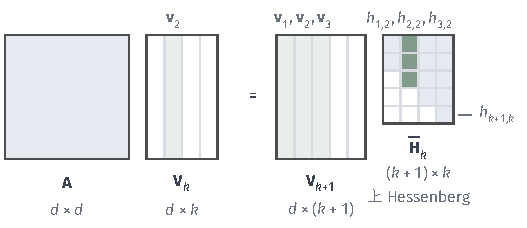
\includegraphics[width=89.098mm]{figures/01-basic-mathematics/03-vectors-matrices-and-multivariate-functions/tikz/c5-arnoldi-relation-shapes/figure.pdf}
  \caption{Arnoldi关系$\bm A\bm V_k=\bm V_{k+1}\overline{\bm H}_k$中各矩阵的形状（示意$d=7$、$k=4$）。$\overline{\bm H}_k$的非零元（浅蓝）只出现在主对角线、其上方和紧邻的下次对角线上，是上Hessenberg矩阵，末行只剩$h_{k+1,k}$。绿色标出第$j=2$列：$\bm A\bm v_2$只用到$\bm v_1,\bm v_2,\bm v_3$，系数是$\overline{\bm H}_k$第2列的前三个元素。}
  \label{fig:ls-arnoldi-relation-shapes}
\end{figure}

左乘$\bm V_k^\top$，并用$\bm V_k^\top\bm V_k=\bm I$与$\bm V_k^\top\bm v_{k+1}=\bm 0$，得
\begin{equation}
 \bm H_k=\bm V_k^\top\bm A\bm V_k .
 \label{eq:ls-arnoldi-projection}
\end{equation}
所以$\bm H_k$是$\bm A$在$\mathcal K_k$上的投影：若$\bm z=\bm V_k\bm y$是子空间中的向量，则$\bm A\bm z$在子空间中的分量的坐标为$\bm H_k\bm y$，伸出子空间的部分只沿$\bm v_{k+1}$一个方向，大小由$h_{k+1,k}$记录。

图中$\bm V_{k+1}$只比$\bm V_k$多一列，而$\overline{\bm H}_k$只有$k+1$行：$d$维矩阵在子空间上的作用，就这样被压缩成一个$k$阶的上Hessenberg矩阵。

\paragraph{正确性}
上面的论证用到了“此前各步的基已经标准正交”。下面的定理用归纳法确认这一点，并给出终止的情形。

\begin{theorem}[Arnoldi关系]
\label{thm:ls-arnoldi-relation}
在精确算术下按式~\eqref{eq:ls-arnoldi-coefficients}与\eqref{eq:ls-arnoldi-normalize}执行$k$轮Arnoldi正交化，且前$k-1$轮的$h_{j+1,j}$均非零。若$h_{k+1,k}\ne0$，则$\bm v_1,\ldots,\bm v_{k+1}$标准正交，$\bm v_1,\ldots,\bm v_j$张成$\mathcal K_j$（$j\le k+1$），关系~\eqref{eq:ls-arnoldi-relation}成立，并且$\bm H_k=\bm V_k^\top\bm A\bm V_k$。若$h_{k+1,k}=0$，则$\bm v_1,\ldots,\bm v_k$标准正交，$\bm A\bm V_k=\bm V_k\bm H_k$，$\mathcal K_k$在$\bm A$下不变；$\bm A$非奇异时精确解$\bm x_\star$属于$\bm x_0+\mathcal K_k$。
\end{theorem}

\begin{proof}
依次证明正交性、张成关系与矩阵关系，最后处理子空间不再扩张的情形。

\emph{正交性。}对$j$归纳，设$\bm v_1,\ldots,\bm v_j$标准正交。第$i$次扣除后$\bm w\perp\bm v_i$，此后扣除的方向$\bm v_{i+1},\ldots,\bm v_j$都与$\bm v_i$正交，不破坏这一关系，所以最终余项与$\bm v_1,\ldots,\bm v_j$都正交。$h_{j+1,j}\ne0$时归一化得到单位向量$\bm v_{j+1}$，与前$j$个正交。

\emph{张成与矩阵关系。}$\bm v_1\in\mathcal K_1$；若$\bm v_1,\ldots,\bm v_j\in\mathcal K_j$，则
\[
 \bm v_{j+1}\in\operatorname{span}\{\bm A\bm v_j,\bm v_1,\ldots,\bm v_j\}\subseteq\mathcal K_{j+1},
\]
$j+1$个标准正交向量落在维数不超过$j+1$的$\mathcal K_{j+1}$中，因而张成它。由式~\eqref{eq:ls-arnoldi-normalize}，扣除完毕后的余项就是$h_{j+1,j}\bm v_{j+1}$，把扣除的分量加回即得列关系~\eqref{eq:ls-arnoldi-column}，并排写出即是式~\eqref{eq:ls-arnoldi-relation}。左乘$\bm V_k^\top$，并用$\bm V_k^\top\bm V_k=\bm I$与$\bm V_k^\top\bm v_{k+1}=\bm 0$，得$\bm H_k=\bm V_k^\top\bm A\bm V_k$。

\emph{不再扩张的情形。}若$h_{k+1,k}=0$，第$k$列成为$\bm A\bm v_k=\sum_{i\le k}h_{i,k}\bm v_i$，于是$\bm A\bm V_k=\bm V_k\bm H_k$，$\bm A\mathcal K_k\subseteq\mathcal K_k$。$\bm A$非奇异时它在有限维空间$\mathcal K_k$上是单射，因而也是满射；$\bm r_0\in\mathcal K_k$，故有$\bm z\in\mathcal K_k$使$\bm A\bm z=\bm r_0$，$\bm x_\star=\bm x_0+\bm z$。
\end{proof}

$\mathcal K_k$的维数不超过$d$，所以至多$d$轮出现$h_{k+1,k}=0$。这时精确解已在候选集合中，使用这组基的求解器在这一步得到精确解，但仍须用原残差确认。

\paragraph{数值敏感度}
有限精度下基的正交性会逐渐损失，判断与补救办法沿用第~\ref{sec:ls-qr-method}节对修正Gram--Schmidt的讨论，必要时按“每轮的更新”所述再正交化。再正交化要用到全部已保存的基向量，Arnoldi正交化本来就保存它们，所以这一补救的代价只是多做一遍投影。

\paragraph{计算代价}
每轮一次$\bm A$乘向量。第$j$轮的扣除要作$j$次内积与$j$次向量更新，约$4dj$次浮点运算，$k$轮合计约$2dk^2$次；保存$\bm V_{k+1}$约需$(k+1)d$个数。两者都随轮数增长，原因是整组基都要保存并参与扣除。本过程只负责生成候选空间，收敛快慢由调用它的求解器在子空间中采用的选解准则决定。

\subsection{应用}
\label{sec:ls-arnoldi-application}

有了基与投影矩阵，就可以在子空间中求解方程。把近似写成
\[
 \bm x_k=\bm x_0+\bm V_k\bm y ,
\]
$\bm y\in\mathbb R^k$是子空间中的坐标。由$\bm r_0=\lVert\bm r_0\rVert_2\bm v_1=\bm V_{k+1}\lVert\bm r_0\rVert_2\bm e_1$与关系~\eqref{eq:ls-arnoldi-relation}，残差可以写成
\begin{equation}
 \bm r_0-\bm A\bm V_k\bm y=\bm V_{k+1}\bigl(\lVert\bm r_0\rVert_2\bm e_1-\overline{\bm H}_k\bm y\bigr),
 \label{eq:ls-arnoldi-residual-coordinates}
\end{equation}
其中$\bm e_1\in\mathbb R^{k+1}$。$d$维的残差由此用$k+1$个坐标表示出来。第~\ref{sec:ls-krylov-selection-criteria}节的准则都可以在这个小问题上实现。

按Galerkin条件，要求残差与$\mathcal K_k$正交，即$\bm V_k^\top(\bm r_0-\bm A\bm V_k\bm y)=\bm 0$。由$\bm H_k=\bm V_k^\top\bm A\bm V_k$，这就是$k$阶上Hessenberg方程组
\begin{equation}
 \bm H_k\bm y=\lVert\bm r_0\rVert_2\,\bm e_1 ,
 \label{eq:ls-arnoldi-galerkin-system}
\end{equation}
这里$\bm e_1\in\mathbb R^k$。

不过对非对称矩阵，Galerkin条件没有极小性，$\bm H_k$也可能奇异。按极小残差条件，则因$\bm V_{k+1}$的列标准正交、不改变长度，在子空间中求残差最小的坐标化为$(k+1)\times k$的小型最小二乘问题
\begin{equation}
 \min_{\bm y}\bigl\lVert\lVert\bm r_0\rVert_2\bm e_1-\overline{\bm H}_k\bm y\bigr\rVert_2 ,
 \label{eq:ls-arnoldi-minimal-residual-problem}
\end{equation}
它对任何非奇异的$\bm A$都有唯一解。这就是GMRES（第~\ref{sec:ls-gmres}节）的做法；$\overline{\bm H}_k$是上Hessenberg矩阵，每增加一列只需一次新的Givens旋转就能延续三角化。

这两种用法都要用$\bm V_k$还原$\bm x_k$，整组基须一直保存，存储与正交化工作随步数增长。实际计算因此常在做满$m$步后停下，以当前近似为新起点重新开始生成基，即\emph{重启}；它限制了存储，代价是失去跨周期的最优性。
